% Chapter 7

\chapter{Resultados} % Main chapter title

\label{Chapter7} % Change X to a consecutive number; for referencing this chapter elsewhere, use \ref{ChapterX}

El objetivo de este capítulo fue el de brindar resultados para distintos escenarios de interés, con el fin de dar comparaciones analíticas con base en la variación de los parámetros de entrada del simulador.

%----------------------------------------------------------------------------------------
%	SECTION 
%----------------------------------------------------------------------------------------

\section{Escenario I} % Simulación con un solo un TTI - FER
\subsection{Descripción del escenario}
Este escenario se concentró en obtener resultados para un solo intervalo de tiempo de transmisión (TTI), con el fin de analizar el rendimiento del modelo de despliegue de UE y el modelo de canal en conjunto con NOMA y evaluar su rendimiento.
Se simuló el rendimiento de \textit{multitone} con diferentes clases de potencia para los dispositivos MTC y con diferentes tamaños de grupos ($kmax$) pero su desempeño no resultó ser importante ya que resultaba ser similar al de singletone. Por este motivo los resultados con la propuesta multitone no se reportaron. Sin embargo, en estos resultados se implementó un modo de operación hibrido donde se adoptó un modo de operación multitone solamente cuando el número de dispositivos es menor al número de grupos (48), esto con la finalidad de no desperdiciar recursos. Y singletone en los demás casos.
También es importante señalar que la relación entre dispositivos mMTC y uRLLC es de 3 a 1.
\subsection{Parámetros de entrada}
De acuerdo con los parámetros generales del modelo de sistema [véase Tabla~\ref{tab:ParametrosGral}], los criterios considerados para este escenario fueron los siguientes:
\begin{itemize} 
	\item $k_{max} \to $ 1, 2 , 3 y 4 grupos
	\item $p_{m}^{s} \to$ 23, 20, 14 dBm
\end{itemize}

\subsection{Resultados obtenidos}
En primera instancia, en el capítulo anterior se analizó el histograma de las pérdidas de canal, del Modelo CI y también del Modelo de canal que proponen en el artículo \parencite{Shahini2019} , de acuerdo con los histogramas se tiene que el valor promedio de las perdidas [dB] en el Modelo CI son de 80.35 dBs. En contrario con las pérdidas del modelo de canal del artículo, tienen un valor promedio de 74.67 dBs. Es decir nuestro canal tiene 3.7 (5.68 dBs) veces más perdidas en comparación del canal que se implementa en \parencite{Shahini2019}, por lo que se espera que el rendimiento sea menor, esto se puede observar en la Figura\ref{fig: NOMA_comprobacion_CI} donde se observa que en el caso de 192 usuarios el desempeño de la simulación del artículo es aproximadamente 140 usuarios, es decir 73\% de los usuarios alcanzan su tasa objetivo. Por el contrario en la evaluación de la simulación con el modelo de canal CI en NOMA se obtiene que aproximadamente 115 usuarios alcanzan su tasa objetivo, es decir, un 60\%. Hay un impacto del canal CI de aproximadamente 13\% del desempeño en comparación con el canal propuesto en \parencite{Shahini2019}.\newline


\begin{figure}[th]
    \centering
    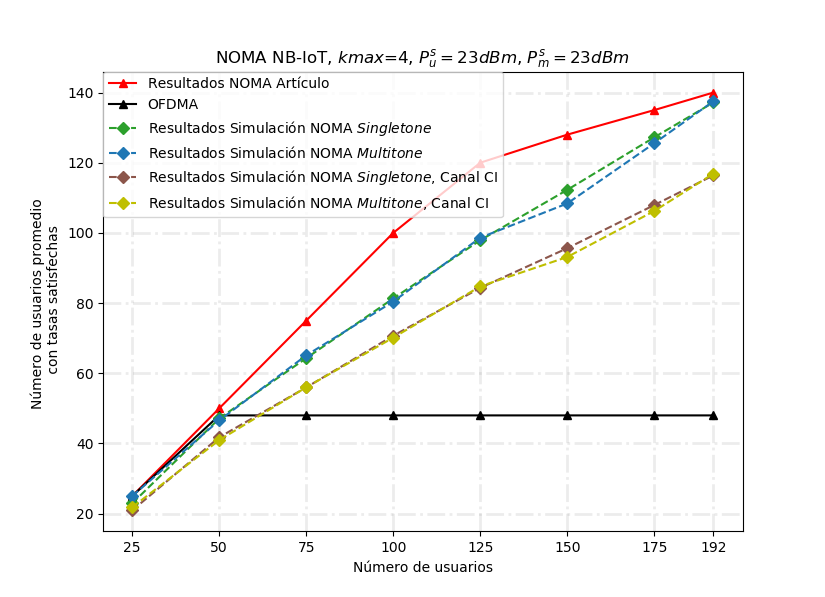
\includegraphics[scale=.7]{Figures/ResultadosNOMA/NOMA_comprobacion_CI.png}
    \decoRule
    \caption[]{}
    \label{fig:NOMA_comprobacion_CI}
\end{figure}

En la Figura~\ref{ NOMA_evaluacion_K_Pm_Variable_3D } se evaluó el número de usuarios que alcanzaron su tasa objetivo, se realizaron comparaciones con respecto a tres tipos de clase de potencia para los mMTC y un variable número de dispositivos por grupo (kmax).\newline

\begin{figure}[th]
    \centering
    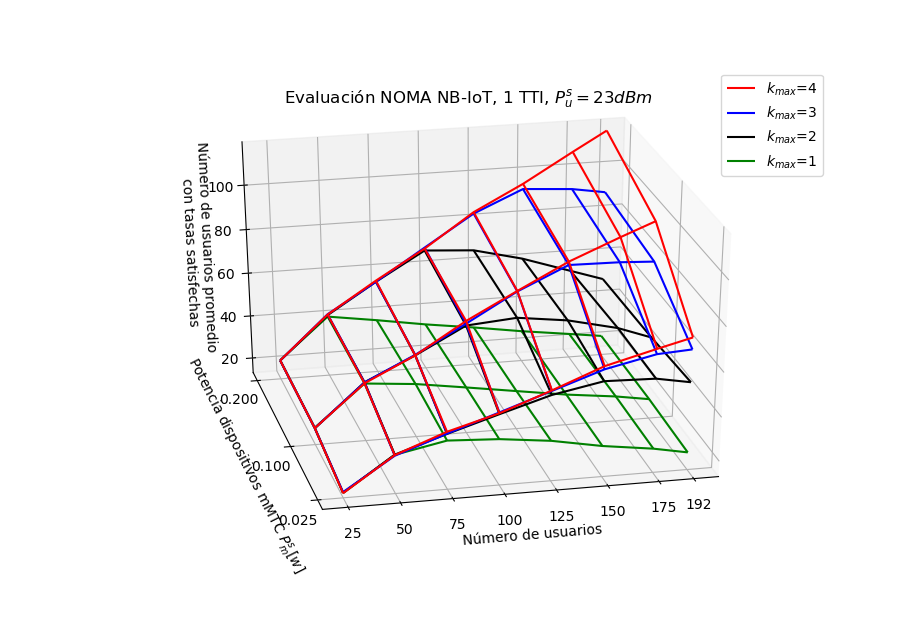
\includegraphics[scale=.7]{Figures/ResultadosNOMA/NOMA_evaluacion_K_Pm_Variable_3D.png}
    \decoRule
    \caption[]{}
    \label{fig:NOMA_evaluacion_K_Pm_Variable_3D}
\end{figure}

Empezando con kmax = 4, se puede observar que entre menor es la potencia de los dispositivos mMTC, el rendimiento de usuarios que alcanzan su tasa objetivo va decayendo y esto es por que al bajar su potencia los dispositivos mMTC varios de ellos comienzan a tener dificultades para alcanzar su tasa objetivo. Si se analiza el caso de 192 usuarios el desempeño con una potencia de usuarios MTC de 23dBm es de aproximadamente 115 usuarios que alcanzan su tasa objetivo, es decir, un 60\%. Y cuando la potencia de usuarios mMTC de 14dBm, 73 dispositivos alcanzan su tasa objetivo, un 38\%. Es decir el rendimiento decrece un 22\% de una potencia de 23 a 14 dBm.\newline

Con kmax=3, vemos que el rendimiento en general decae cuando son 150 usuarios y es porque en este caso, el máximo de usuarios que pueden ser atendidos es de 144, por lo que en los casos de 175 y 192 usuarios el rendimiento va bajando esto es por la relación 3 a 1 que se propuso en los parámetros de entrada. También conforme se baja la potencia de los dispositivos mMTC, se puede ver que el rendimiento decae. Si se analiza el caso de 150 usuarios el desempeño con una potencia de usuarios MTC de 23dBm es de aproximadamente 89 usuarios que alcanzan su tasa objetivo, es decir, un 59\%. Y cuando la potencia de usuarios mMTC de 14dBm, 67 dispositivos alcanzan su tasa objetivo, un 44\%. Es decir el rendimiento decrece un 15\% de una potencia de 23 a 14 dBm.\newline

Con kmax=2, se observa que el rendimiento en general decae cuando son 100 usuarios y es porque en este caso, el máximo de usuarios que pueden ser atendidos es de 96, por lo que en los casos mayores a 100 usuarios el rendimiento va bajando esto igualmente es por la relación 3 a 1. De igual manera también se puede ver que el rendimiento decae cuando se baja la potencia de los dispositivos mMTC. Si se analiza el caso de 100 usuarios el desempeño con una potencia de usuarios MTC de 23dBm es de aproximadamente 53 usuarios que alcanzan su tasa objetivo, es decir, un 53\%. Y cuando la potencia de usuarios mMTC de 14dBm, 49 dispositivos alcanzan su tasa objetivo, un 49\%. Es decir el rendimiento decrece solamente 4\% de una potencia de 23 a 14 dBm.\newline

Con kmax=1, de la misma forma se observa que el rendimiento en general decae cuando son 50 usuarios y es porque en este caso, el máximo de usuarios que pueden ser atendidos es de 48, por lo que en los casos mayores a 100 usuarios el rendimiento va bajando esto igualmente es por la relación 3 a 1. También conforme se baja la potencia de los dispositivos mMTC, se puede ver que el rendimiento no decae de manera significativa como lo fue en los otros casos. 

En las siguientes figuras se evaluo la misma métrica del número de usuarios que alcanzan su tasa objetivo pero ahora desde la perspectiva de cuantos de estos son uRLLC y cuantos mMTC.\newline


\begin{figure}[th]
    \centering
    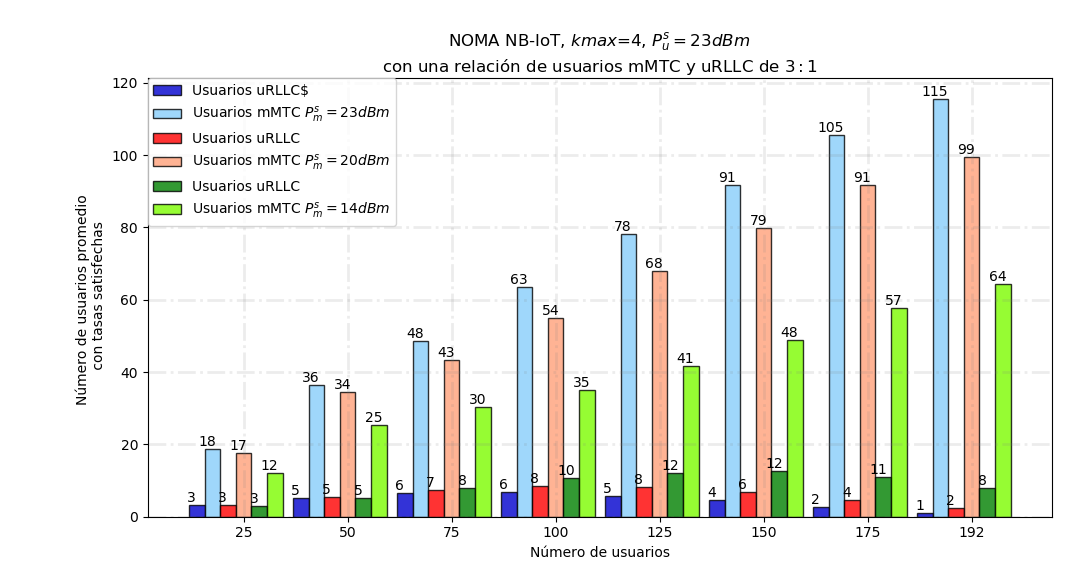
\includegraphics[scale=.6]{Figures/ResultadosNOMA/Kmax4_DiferentesPM.png}
    \decoRule
    \caption[]{}
    \label{fig:Kmax4_DiferentesPM}
\end{figure}

\begin{figure}[th]
    \centering
    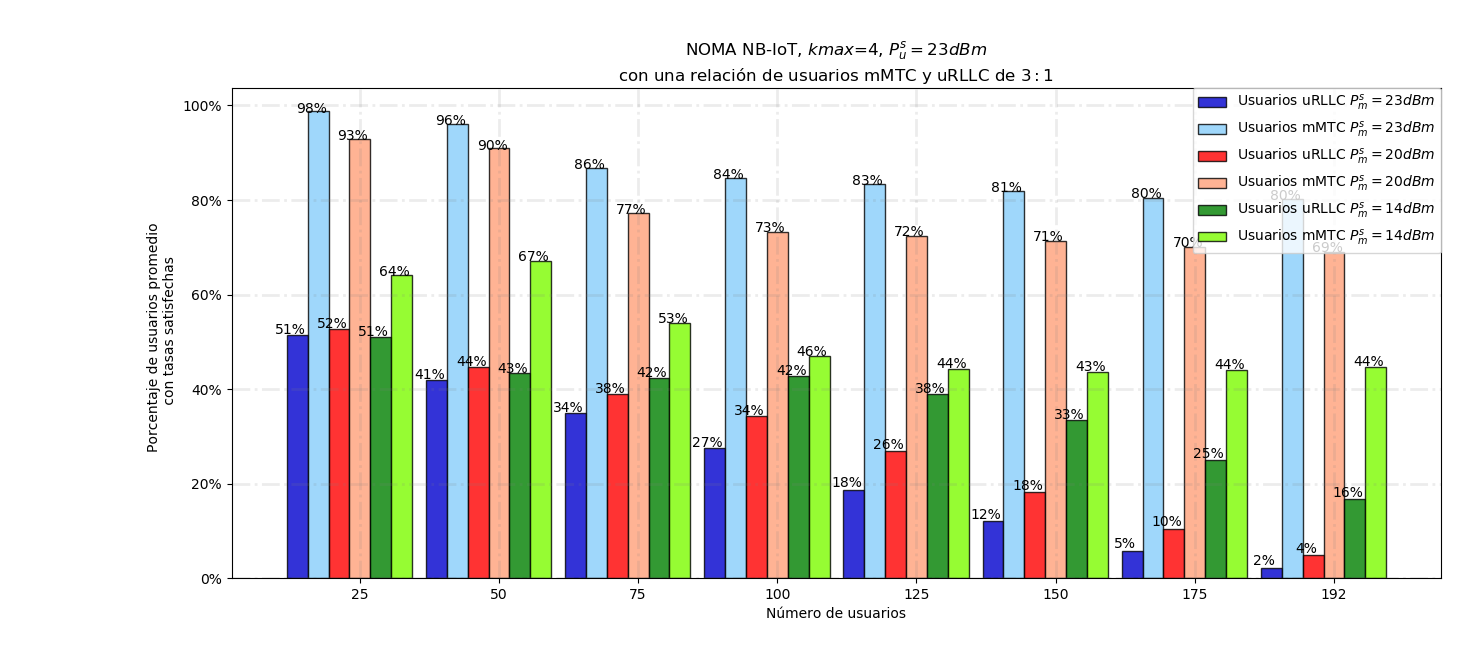
\includegraphics[scale=.6]{Figures/ResultadosNOMA/Kmax4_DiferentesPM_Porcentual.png}
    \decoRule
    \caption[]{}
    \label{fig:Kmax4_DiferentesPM_Porcentual}
\end{figure}


La Figura~\ref{fig:Kmax4_DiferentesPM} representa graficas de barras acerca de la evaluación del número de usuarios mMTC y uRLLC que alcanzaron su tasa objetivo en un TTI, esto con un Kmax = 4 (192 usuarios como máximo), se realizaron comparaciones con diferentes potencias de los dispositivos mMTC. Igualmente, En la Figura~\ref{fig:Kmax4_DiferentesPM_Porcentual} se representan graficas de barras acerca de la evaluación del número de usuarios mMTC y uRLLC que alcanzaron su tasa objetivoI, pero esta vez mostrando el porcentaje de dispositivos mMTC y uRLLC que alcanzan su tasa objetivo, de acuerdo a la relación 3 a 1 que se planteó en los parámetros de entrada.\newline

Primeramente, con una potencia de 23dBm para los dispositivos mMTC (color azul), se observa que entre mayor sea el número de usuarios la correlación entre dispositivos uRLLC y mMTC que alcanzan su tasa se va volviendo más desproporcional, esto se puede ver más claramente en la Figura~\ref{ Kmax4_DiferentesPM_Porcentual}. P. Ej., cuando son 25 usuarios la proporción uRLLC y mMTC es de 51\%- 98\% respectivamente y cuando el número de usuarios aumenta a 192 usuarios la proporción uRLLC y mMTC es de 2\%- 80\% respectivamente (esto es con base en la relación 3 a 1). Como se observa la proporción de uRLLC y mMTC que alcanzan su tasa es muy desproporcional o injusta.\newline

En los casos en donde la potencia de los usuarios mMTC es menor a la de los uRLLC, se observa una mejor proporción entre los tipos de dispositivos. P. Ej. Con una potencia de 14dBm para los dispositivos mMTC (color verde) la proporción de dispositivos uRLLC y mMTC es de 51\%- 64\% respectivamente y cuando el número de usuarios aumenta a 192 usuarios la proporción uRLLC y mMTC es de 16\%- 44\% respectivamente (esto es con base en la relación 3 a 1). Como se observa la proporción de uRLLC y mMTC que alcanzan su tasa es más proporcional comparado con el análisis de potencia de los usuarios mMTC en 23 dBm. \newline


\begin{figure}[th]
    \centering
    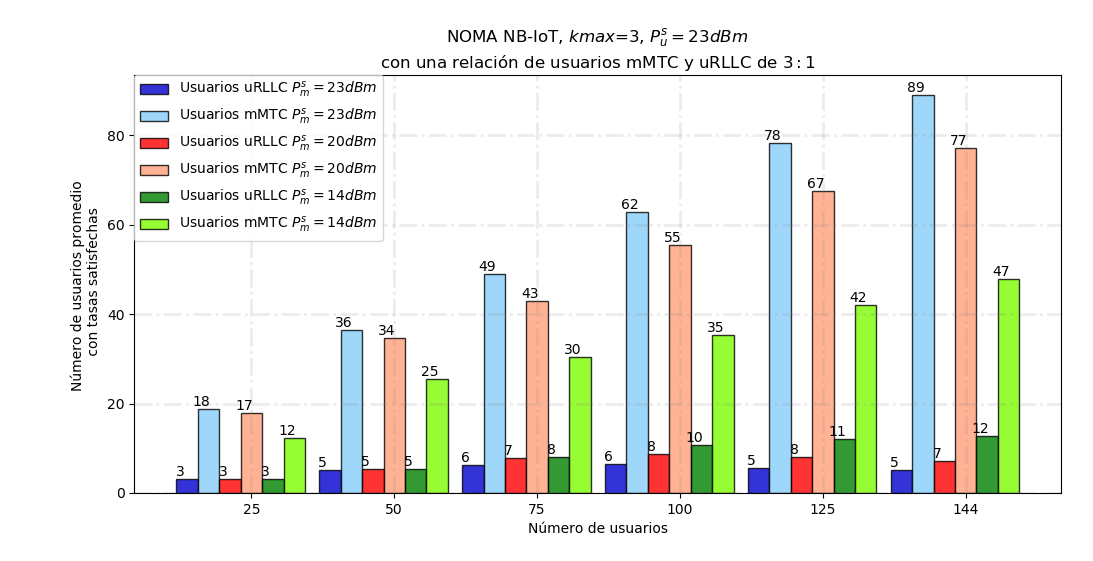
\includegraphics[scale=.6]{Figures/ResultadosNOMA/Kmax3_DiferentesPM.png}
    \decoRule
    \caption[]{}
    \label{fig:Kmax3_DiferentesPM}
\end{figure}

\begin{figure}[th]
    \centering
    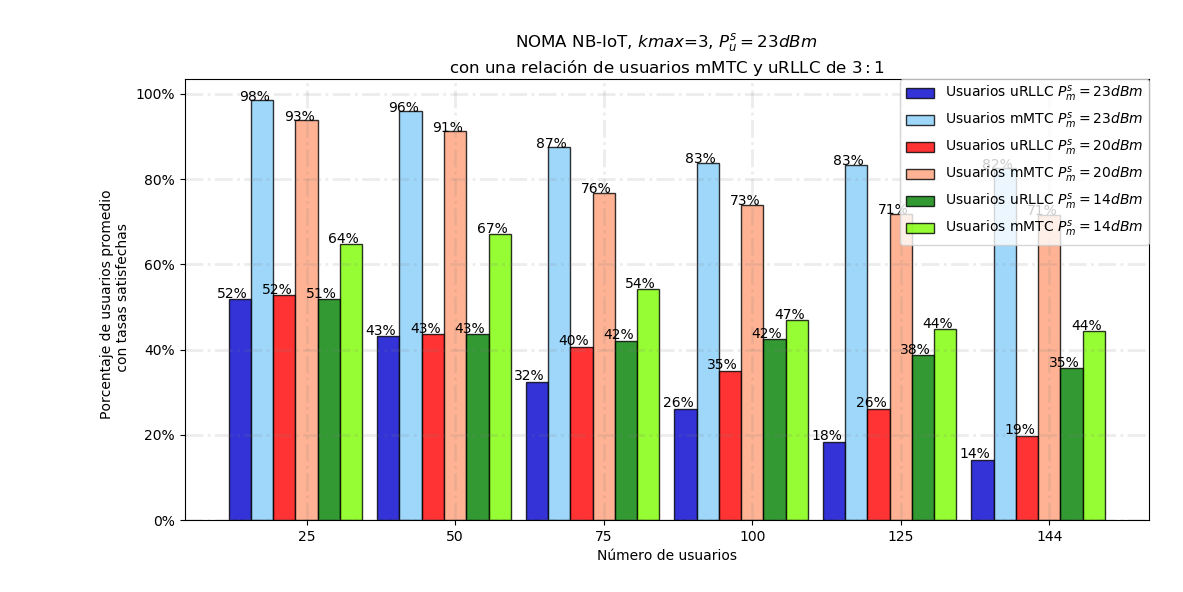
\includegraphics[scale=.6]{Figures/ResultadosNOMA/Kmax3_DiferentesPM_Porcentual.png}
    \decoRule
    \caption[]{}
    \label{fig:Kmax3_DiferentesPM_Porcentual}
\end{figure}


Las Figuras~\ref{fig:Kmax3_DiferentesPM} y ~\ref{fig:Kmax3_DiferentesPM_Porcentual} representan graficas de barras acerca de la evaluación del número de usuarios mMTC y uRLLC que alcanzaron su tasa objetivo en un TTI, esto con un Kmax = 3 (144 usuarios como máximo), se realizaron comparaciones con diferentes potencias de los dispositivos mMTC.

Primeramente, con una potencia de 23dBm para los dispositivos mMTC (color azul), se observó que de igual manera, entre mayor sea el número de usuarios la correlación entre dispositivos uRLLC y mMTC que alcanzaban su tasa se va volviendo más desproporcional, esto se puede ver más claramente en la Figura~\ref{fig:Kmax3_DiferentesPM_Porcentual}. P. Ej., cuando son 25 usuarios la proporción uRLLC y mMTC es de 52\%- 98\% respectivamente y cuando el número de usuarios aumenta a 144 usuarios la proporción uRLLC y mMTC es de 14\%- 82\% respectivamente (esto es con base en la relación 3 a 1). Como se observa la proporción de uRLLC y mMTC que alcanzan su tasa sigue siendo desproporcional pero no tanto comparado con kmax = 4, esto es porque menos dispositivos son agrupados.\newline

En los casos en donde la potencia de los usuarios mMTC es menor a la de los uRLLC, se observó de la misma manera que estos obtienen una mejor proporción. P. Ej. Con una potencia de 14dBm para los dispositivos mMTC (color verde) la proporción de dispositivos uRLLC y mMTC es de 51\%- 64\% respectivamente y cuando el número de usuarios aumenta a 144 usuarios, la proporción uRLLC y mMTC es de 35\%- 44\% respectivamente (esto es con base en la relación 3 a 1). Como se observa la proporción de uRLLC y mMTC que alcanzan su tasa es más proporcional comparado con el análisis de potencia de los usuarios mMTC en 23 dBm. \newline



\begin{figure}[th]
    \centering
    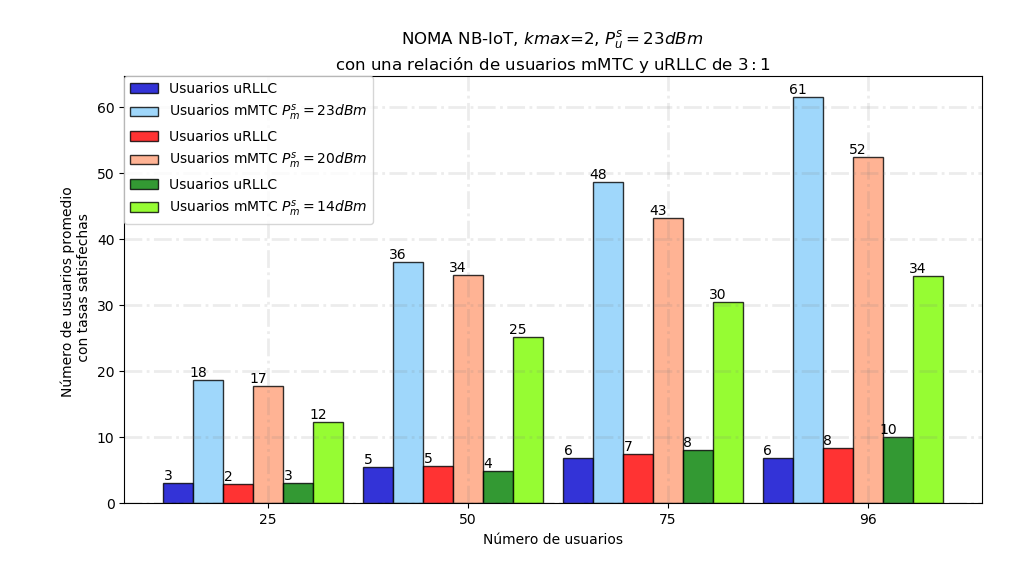
\includegraphics[scale=.5]{Figures/ResultadosNOMA/Kmax2_DiferentesPM.png}
    \decoRule
    \caption[]{}
    \label{fig:Kmax2_DiferentesPM}
\end{figure}

\begin{figure}[th]
    \centering
    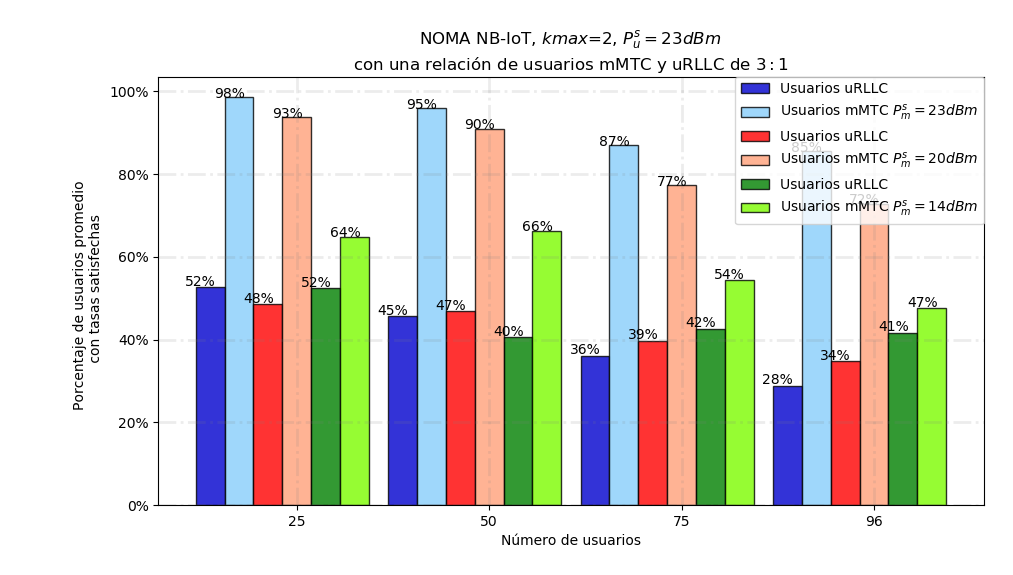
\includegraphics[scale=.5]{Figures/ResultadosNOMA/Kmax2_DiferentesPM_Porcentual.png}
    \decoRule
    \caption[]{}
    \label{fig:Kmax2_DiferentesPM_Porcentual}
\end{figure}

Las Figuras~\ref{fig:Kmax2_DiferentesPM} y ~\ref{fig:Kmax2_DiferentesPM_Porcentual} representan graficas de barras acerca de la evaluación del número de usuarios mMTC y uRLLC que alcanzaron su tasa objetivo en un TTI, esto con un Kmax = 2 (96 usuarios como máximo), se realizaron comparaciones con diferentes potencias de los dispositivos mMTC.\newline

Primeramente, con una potencia de 23dBm para los dispositivos mMTC (color azul), se observó que de igual manera, entre mayor sea el número de usuarios la correlación entre dispositivos uRLLC y mMTC que alcanzaban su tasa se va volviendo más desproporcional, esto se puede ver más claramente en la Figura~\ref{fig:Kmax2_DiferentesPM_Porcentual}. P. Ej., cuando son 25 usuarios la proporción uRLLC y mMTC es de 52\%- 98\% respectivamente y cuando el número de usuarios aumenta a 96 usuarios la proporción uRLLC y mMTC es de 28\%- 85\% respectivamente (esto es con base en la relación 3 a 1). Como se observa la proporción de uRLLC y mMTC que alcanzan su tasa sigue siendo desproporcional pero no tanto comparado con kmax = 3, esto es porque menos dispositivos son agrupados.\newline

En los casos en donde la potencia de los usuarios mMTC es menor a la de los uRLLC, se observó de la misma manera que estos obtienen una mejor proporción. P. Ej. Con una potencia de 14dBm para los dispositivos mMTC (color verde) la proporción de dispositivos uRLLC y mMTC es de 52\%- 64\% respectivamente y cuando el número de usuarios aumenta a 144 usuarios, la proporción uRLLC y mMTC es de 41\%- 47\% respectivamente (esto es con base en la relación 3 a 1). Como se observa la proporción de uRLLC y mMTC que alcanzan su tasa es más proporcional comparado con el análisis de potencia de los usuarios mMTC en 23 dBm. \newline


Para finalizar esta sección, se pudo examinar que de la Figura~\ref{fig:NOMA_evaluacion_K_Pm_Variable_3D}, se concluye que entre menor sea la potencia de los mMTC, el número de dispositivos que alcanzan su tasa objetivo es menor, pero al hacer el análisis de las gráficas de barras enfocadas en cuantos dispositivos uRLLC y mMTC fueron los que alcanzaron su tasa, se observó que la proporción de los tipos de dispositivos mejoraba.


%----------------------------------------------------------------------------------------
%	SECTION 
%----------------------------------------------------------------------------------------

\section{Escenario II} % Simulación completa con tráfico - 

Este segundo escenario pone a prueba la capacidad que tiene el programa principal \textbf{Simulador de modelos de tráfico para nodos IoT en una red celular de 5G}, de generar resultados que permitan comparar el efecto que tiene establecer distintos parámetros de la red en el \textit{throughput} del sistema y en el porcentaje de dispositivos que cumplen su tasa deseada. \newline

\subsection{Descripción del escenario}

En este este escenario se consideraron únicamente los dispoitivos de tipo URLLC y los llamados Otros dispositivos mMTC, esto para facilitar el cumplir con la relación de 3 a 1 entre ambos tipos de dispositivos. Entonces en el programa \textbf{Generador de tráfico IoT} se generó tráfico dentro de una célula de radio igual a 200 metros. La distribución de usuarios se hizo con la opción PPP y se establecieron las intensidades de la siguiente forma: La intensidad de los dispositivos mMTC se fijo en 0.3 $dispositivos/m^2$ y la de los dispositivos URLLC se fijo en 0.1 $dispositivos/m^2$. La relación de dispositivos se eligió 3 a 1 para después fijar las tasas de nacimientos de paquetes y de alarmas idénticas en ambos tipos de servicios y garantizar que el tráfico ofrecido al sistema conserve esa relación. La tasa de nacimiento de paquetes es $\lambda_{normal} = 0.0167 paquetes/seg.$ y la de nacimiento de alarmas es $\lambda_{alarma} = 0.1 alarmas/seg.$ para ambos tipos de dispositivos. Finalmente, las características en las que se transmiten las alarmas son compartidas también entre ambos dispositivos: $velocidad_{alarma} = 500 m/s$ y modelo de propagación espacial = \textit{Rised-cosine window} con $d_{th}=200$ y $d_{th}=100$. \newline

De manera que virtualmente, ambos tipos los dispositivos generan tráfico del mismo tipo, pero al haber 3 veces más dispositivos mMTC, en los algoritmos NOMA se conservará en promedio esta relación.

El tráfico generado por el \textbf{Generador de tráfico IoT} correspondió a 10 segundos y la iteración seleccionada para ser evaluada por el simulador de eventos discretos contenía 2 alarmas, una para cada tipo de dispositivo, lo que es el promedio esperado, dado que $\lambda_{alarma} = 0.1 alarmas/seg.$. Se seleccionó esta iteración por ser una buena representación de los parámetros ingresados. Finalmente se inició la simulación con 48 dispositivos ya utilizando el canal, 26 dispositivos mMTC y 12 URLLC, esto para que el sistema se encontrara ya en un equilibrio de operación.

\subsection{Parámetros de entrada}

La instancia de tráfico utilizada como entrada del simulador de eventos discretos, comprendía $37541$ dispositivos mMTC y $12611$ dispositivos URLLC. El tiempo de la simulación se fijo en $10$ segundos y las potencias máximas de transmisión en los dispositivos se fijaron como $23dBm$ para los URLLC y $20dBm$ para los mMTC. Finalmente se usó $d0=1m$, $PLE=2.0$ y el bloque de frecuencias que inicia en $2Ghz$. 

Se corrieron 4 rutinas en las que se variaron los valores de $k$ desde $1$ hasta $4$.

\subsection{Resultados obtenidos}

Para \textbf{k=1} se obtuvo:\newline
Tráfico ofrecido = $48182.749345 bytes/s$ \newline
Throughput = $31578.300434 bytes/s$ \newline
Probabilidad de bloqueo sin clúster = $36.674849 porciento$ \newline
Tasas no cubiertas URLLC = $25.670367 porciento$ \newline
Tasas no cubiertas URLLC = $17.796712 porciento$ \newline

Para \textbf{k=2} se obtuvo:\newline
Tráfico ofrecido = $48182.749345 bytes/s$ \newline
Throughput = $33391.109178 bytes/s$ \newline
Probabilidad de bloqueo sin clúster = $32.644499 porciento$ \newline
Tasas no cubiertas URLLC = $22.322801 porciento$ \newline
Tasas no cubiertas URLLC = $11.487657 porciento$ \newline

Para \textbf{k=3} se obtuvo:\newline
Tráfico ofrecido = $48182.749345 bytes/s$ \newline
Throughput = $34457.869843 bytes/s$ \newline
Probabilidad de bloqueo sin clúster = $30.363758 porciento$ \newline
Tasas no cubiertas URLLC = $24.560205 porciento$ \newline
Tasas no cubiertas URLLC = $11.829281 porciento$ \newline

Para \textbf{k=4} se obtuvo:\newline
Tráfico ofrecido = $48182.749345 bytes/s$ \newline
Throughput = $35150.834596 bytes/s$ \newline
Probabilidad de bloqueo sin clúster = $28.829673 porciento$ \newline
Tasas no cubiertas URLLC = $24.184458 porciento$ \newline
Tasas no cubiertas URLLC = $11.427156 porciento$ \newline

De los resultados se puede ver que aumentar k también aumenta el \textit{throughput} y reduce la probabilidad de bloqueo por negación de servicio sin comprometer el porcentaje de tasas no cubiertas, pero variar la potencia de transmisión y evaluar más iteraciones de tráfico son necesarias para dar una respuesta definitiva, sin embargo se puede ver que el simulador genera los datos requeridos, y apartir de estos se puede identificar el comportammiento del sistema para distintos parámetros de entrada.